%% Author: Daniel Kaplan
%% Subject: Graphics (distributions)




\providecommand{\HCode}[1]{#1} % dummy, just in case it's PDFlatex
\HCode{<link rel="stylesheet" href="fixSweave.css" type="text/css"
  media="screen" />}
\HCode{<link rel="stylesheet" href="http://dl.dropbox.com/u/5098197/Math135/RGuide/fixSweave.css" type="text/css"
 media="screen" />}

This exercise 
deals with data on weight loss achieved by clients who stayed two weeks
at a weight-loss resort.  The same data  using 
three different
sorts of graphical displays:
a pie chart, a histogram, and a box-and-whiskers plot.  The point of
the exercise is to help you decide which display is the most
effective at presenting information to you. 

In many fields, pie charts are used as ``statistical graphics.''
Here's a pie chart of the weight loss:


\centerline{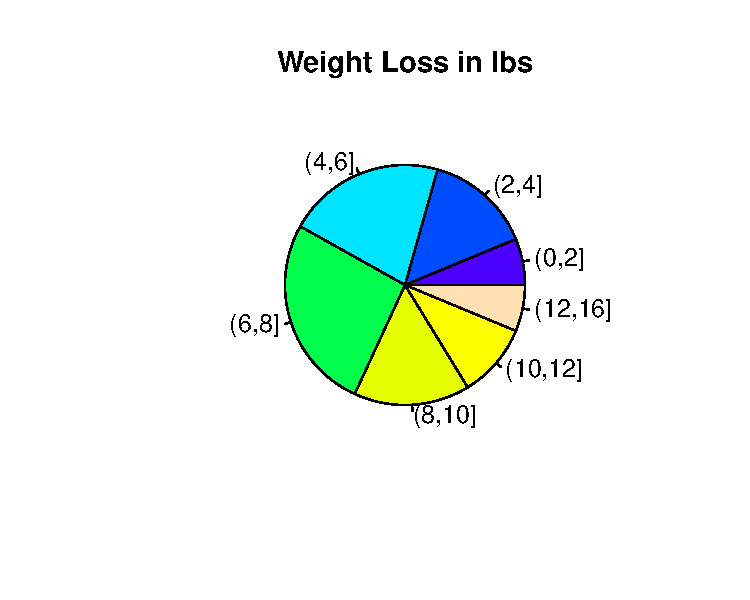
\includegraphics[width=2.5in,trim=35 20 25 0]{Figures/S2008-var2-pie}}

%\centerline{\pnggraphicsfile[width=2in]{weight-loss-pie}{pdf}{40}}


Using the pie graph, answer the following:
\begin{enumerate}[(a)]
\item What's the ``typical'' (median or mean) weight loss?
\SelectSetHoriz{6.8}{3.7,4.2,5.5,6.8,8.3,10.1,12.4}
\item What is the central 50\% coverage interval?\\
\SelectSetHoriz{4.4to8.7}{2.3to6.8,4.2to10.7,4.4to8.7,6.1 to
9.3,5.2to12.1}
\item What is an upper extreme value?
\SelectSetHoriz{16}{10,13,16,18,20}
\end{enumerate}

\begin{AnswerText}
It's very difficult to figure out the answers from the pie chart.
In general, people have a hard time with them, particularly when it
comes to comparing two different pie charts.
\end{AnswerText}

\bigskip

Now to display the data as a histogram.  So that you can't just re-use
your answers from the pie chart, the weights have been 
rescaled into kilograms.


\centerline{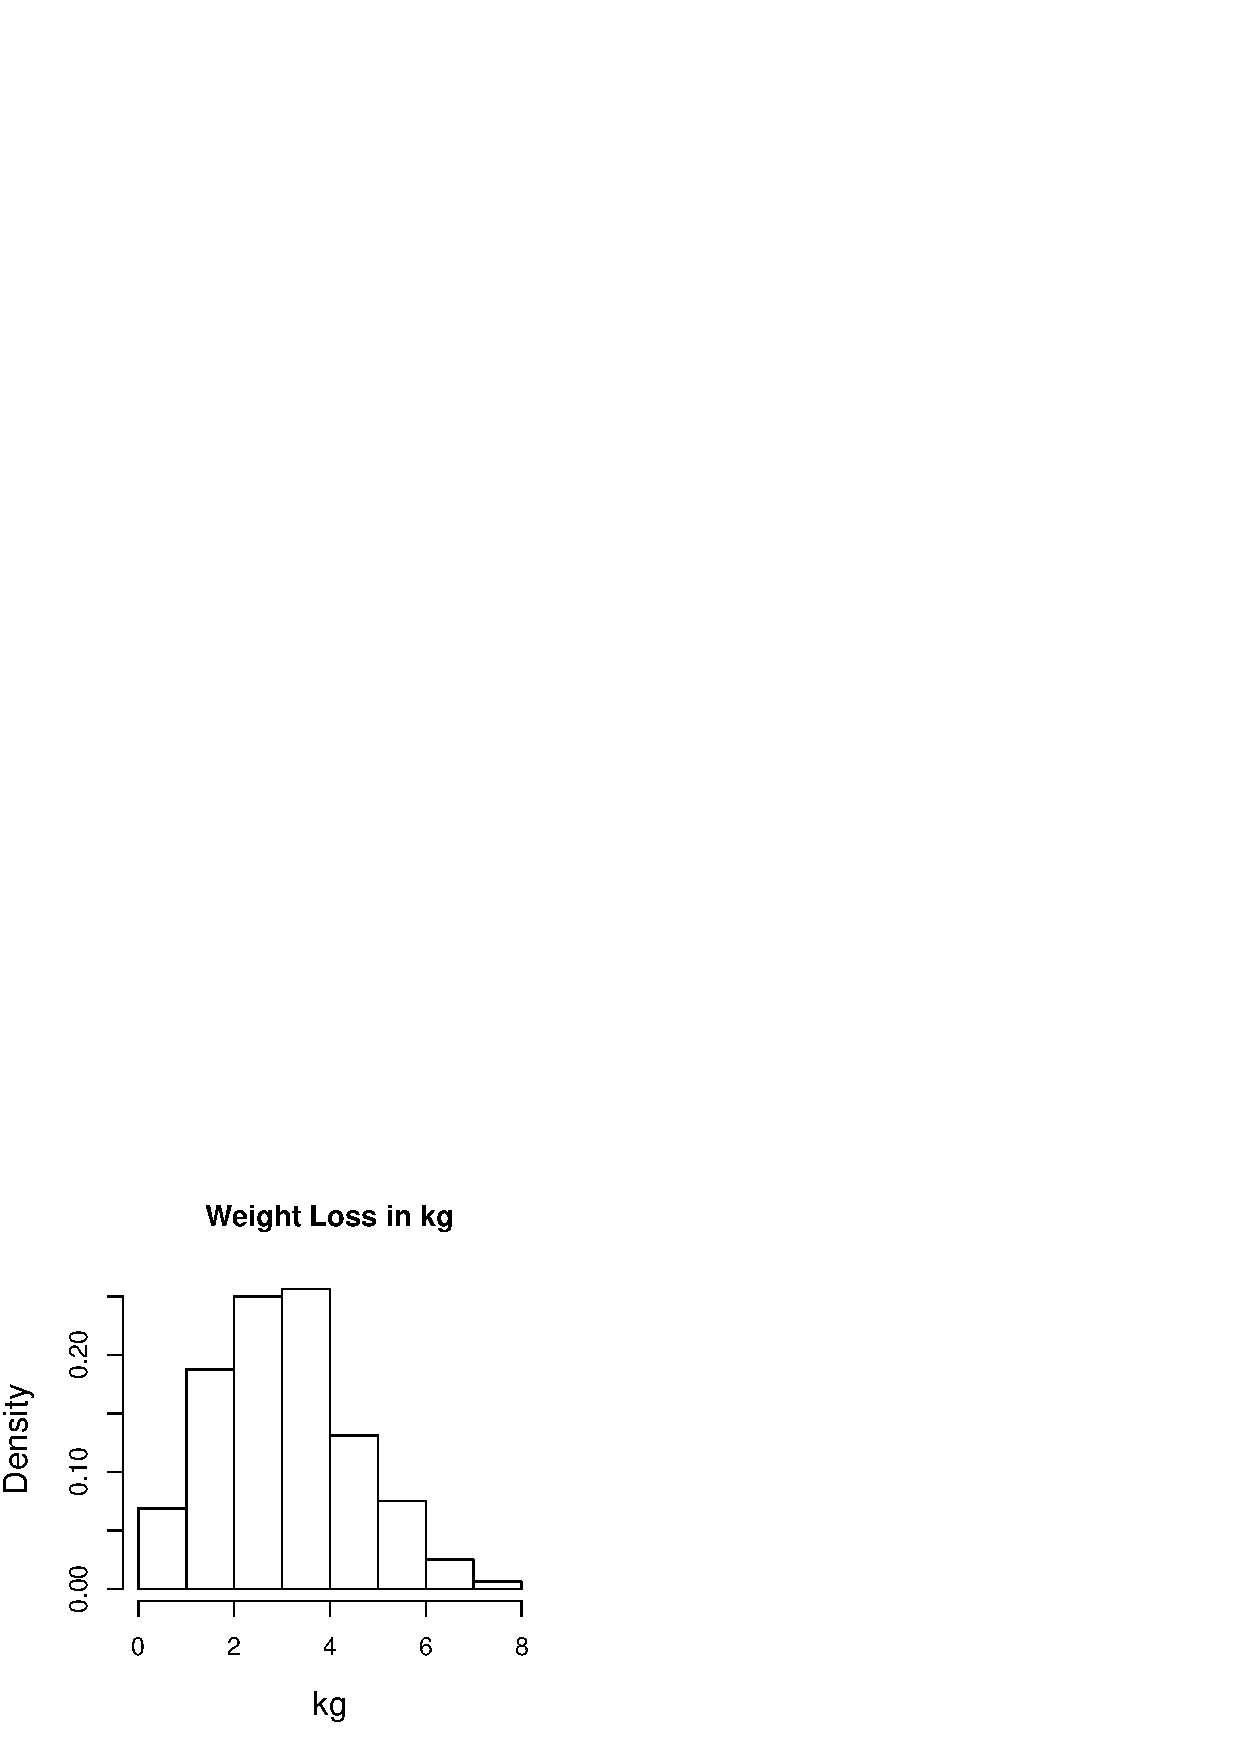
\includegraphics[width=2.5in,trim=35 20 25 0]{Figures/S2008-var2-hist}}
% \centerline{\pnggraphicsfile[width=2in]{weight-loss-hist}{pdf}{50}}

Using the histogram, answer the following:
\begin{enumerate}
\item What's the ``typical'' (median or mean) weight loss?\\
\SelectSetHoriz{3.1}{1.9,2.1,3.1,3.7,4.6,5.6}
\item What is the central 50\% coverage interval?\\
\SelectSetHoriz{2.0to3.9}{1.1to3.3,2.0to4.8,2.0to3.9,2.8 to
4.4,2.5to5.4}
\item What is an upper extreme value?
\SelectSetHoriz{8}{6,8,10,12,14}
\end{enumerate}

\bigskip

Finally, here is a boxplot of the same data.  It's been rescaled into
a traditional unit of weight: stones.


\centerline{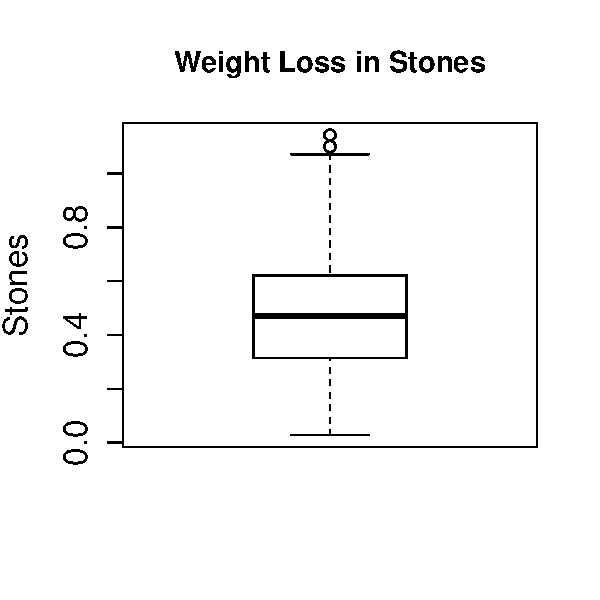
\includegraphics[width=2.5in,trim=35 20 25 0]{Figures/S2008-var2-box}}

%\centerline{\pnggraphicsfile[width=2in]{weight-loss-box}{pdf}{50}}


Using the boxplot, answer the following:
\begin{enumerate}
\item What's the ``typical'' (median or mean) weight loss?\\
\SelectSetHoriz{0.50}{0.20,0.35,0.50,0.68,0.83,1.2}
\item What is the central 50\% coverage interval?\\
\SelectSetHoriz{0.3to0.6}{0.2to0.5,0.3to0.8,0.4to0.8,0.5to0.7,0.3to0.6}
\item What is an upper extreme value?
\SelectSetHoriz{1.1}{0.7,0.9,1.0,1.1,1.3}
\end{enumerate}

\bigskip

Which style of graphic made it easiest to answer the questions?\\
\SelectSetHoriz{no.correct.answer}{pie.chart,histogram,box.plot}

% e-mail May 31, 2008 from 
% Erin Knutson, 
% Media Relations Specialist, 
% Hilton Head Health, 
% w: 843.785.3919 

% The spreadsheet containing weight loss data. 
% [dataset WeightLoss.csv] % in Problems/S2008
% email June 3, 2008 from Courtney Bell, getserious@hhhealth.com


\begin{comment}
w = read.csv('WeightLoss.csv')
ww = subset(w, w$Days==14)
foo = cut( ww$WeightLoss, breaks=c(0,2,4,6,8,10,12,16))
pie(table(foo),main='Weight Loss in lbs',topo.colors(7))
hist( ww$WeightLoss/2.2, main='Weight Loss in kg',
   freq=FALSE,xlab='kg',cex.lab=1.3)
boxplot( ww$WeightLoss/14,ylab='Stones',cex.lab=1.3,cex.axis=1.3,
  main='Weight Loss in Stones')

\end{comment}


